\documentclass[10pt,letterpaper]{article}
\usepackage[letterpaper,margin=1in]{geometry}
\usepackage[T1]{fontenc}
\usepackage{mathptmx}
\usepackage[scaled=0.9]{helvet}
\usepackage{courier}
\usepackage[protrusion=false,expansion=false]{microtype}
\usepackage{amsmath,amssymb,amsthm,booktabs,array,graphicx,xcolor,enumitem}
\usepackage{tikz}
\usetikzlibrary{arrows.meta,positioning,fit}
\usepackage[font=normalsize,labelfont=bf,skip=4pt]{caption}
\usepackage[colorlinks,linkcolor=blue!50!black,citecolor=blue!50!black,urlcolor=blue!50!black]{hyperref}

\newtheorem{proposition}{Proposition}
\newtheorem{lemma}{Lemma}
\newcommand{\sd}{\operatorname{sd}}
\newcommand{\R}{\mathbb{R}}
\newcommand{\REPO}{\url{https://github.com/JSR996/bbb-gnn-permeability}}
\setlength{\tabcolsep}{4pt}
\setlength{\floatsep}{8pt plus 2pt minus 2pt}
\setlength{\textfloatsep}{9pt plus 2pt minus 3pt}
\setlength{\intextsep}{8pt plus 2pt minus 2pt}
\setlength{\parskip}{0pt}
\setlist{nosep}

\title{Group-Relative Reinforcement Learning for Blood--Brain-Barrier Molecule Design:\\
What Restrains Reward Hacking, and What Does Not}
\author{S Hariharan \and J Shrenik Reddy \and Ansa N}
\date{}

\begin{document}
%------------------------------------------------------------------ title page (not counted)
\begin{titlepage}
\maketitle
\thispagestyle{empty}
\begin{center}\textbf{Abstract}\end{center}\vspace{-0.5em}\begin{quote}\noindent
We study a two-stage system for proposing molecules predicted to cross the blood--brain barrier (BBB): a graph-neural-network permeability classifier, reused as a frozen reward for a group-relative policy-optimization (GRPO) generator. Everything is measured at ten seeds on a leak-corrected scaffold protocol. On the classifier side, descriptor fusion and batch normalization are the only components with a resolved gain (+0.0099 and +0.0074 ROC-AUC, jointly +0.0195); the choice of message-passing operator is not resolved, and in-distribution rank does not predict rank on an external holdout ($r=-0.45$, $p=0.16$, 11 models). On the generator side, an unconstrained loop collapses scaffold fraction from $0.72$--$0.80$ to $0.07$--$0.14$ in 200 steps while validity rises to $100\%$ and every metric the loop originally logged looks healthy. Because the group-standardized advantage is blind to the absolute reward level, only quantities that act outside it (a size gate, a fixed invalidity floor, a KL penalty) restrain the collapse; reweighting inside it does not. Replacing the permeability term by a permeability \emph{gate} gives $73\%$ more distinct output on BBBP and cuts reproduction of the training corpus from $88.9\%$ to $68.4\%$, but a replication on B3DB shrinks the gain to $18\%$, with a mechanism: the benefit scales with how badly the policy had memorized its corpus. Against baselines, GRPO significantly improves the quantities in its reward (classifier score $+0.126$, QED $+0.054$) but not an independent drug-likeness composite (CNS-MPO $+0.008$, $p=0.45$). $72.0\%$ of generated molecules are absent from PubChem and the training corpus. The central limitation is unresolved: the BBBP label measures transport, not drug suitability, so a permeability objective rewards small lipophilic solvents. All outputs are hypotheses, not synthesis candidates.
\end{quote}
\vspace{1.5em}
\noindent\textbf{Source code and data (public).} The repository \REPO{} (branch \texttt{ranking-v2}, commit \texttt{0d1e4e85}) holds the classifier and generator code, all committed result tables, run histories and samples, and a README documenting setup and reproduction (\texttt{python -m src.pipeline}). The directory \texttt{paper/} of the repository contains this paper's \LaTeX{} sources, all figures and the scripts that regenerate them. A single supplementary PDF (``Supplement'' below) holds the appendix.
\end{titlepage}

%------------------------------------------------------------------ body (10 pages)
\section{Introduction}
Whether a small molecule crosses the BBB decides if it can act on the central nervous system. Public labelled sets are small: BBBP holds roughly two thousand compounds \cite{martins2012,wu2018} and B3DB about eight thousand \cite{meng2021}. Graph neural networks reach high ranking accuracy on them, and it is natural to reuse a trained network as the reward of a generative model \cite{olivecrona2017}.

That reuse changes the question. A classifier is judged on molecules resembling its training data; a generator queries it on molecules chosen to maximize its output, so any systematic weakness is sought out \cite{manheim2018,skalse2022,gao2022}. This paper documents what happened when we did exactly that, and which interventions worked. Our contributions are:
\begin{enumerate}[leftmargin=*,itemsep=1pt]
\item \textbf{A corrected classifier protocol and a ten-seed comparison} (Section~\ref{sec:clf}). Acyclic molecules were silently excluded from every test fold by the standard Murcko grouping; we fix this, and show most architecture comparisons are within seed noise.
\item \textbf{A group-relative generator with a two-part (hurdle) advantage} and a statement of what a group-standardized update cannot see (Section~\ref{sec:theory}), tested against an unconstrained baseline that collapses (Section~\ref{sec:collapse}).
\item \textbf{A measured account of which anchors work}, including two retractions of our own earlier claims (Sections~\ref{sec:anchors}--\ref{sec:brics}).
\item \textbf{Permeability as a gate, replicated on a second corpus}, with baselines, an out-of-loop judge, a PubChem provenance census and a ranking correction (Section~\ref{sec:gate}).
\end{enumerate}
Section~\ref{sec:limits} states what remains unresolved. All code, result tables and run histories are public: \REPO{} (branch \texttt{ranking-v2}).

\section{Related Work}
\textbf{Graph models of molecules.} GCN \cite{kipf2017}, GraphSAGE \cite{hamilton2017}, GIN \cite{xu2019} and GAT \cite{velickovic2018} are message-passing operators \cite{gilmer2017}; bond-aware variants extend GIN \cite{hu2020}, and the D-MPNN passes messages along directed bonds \cite{yang2019}. MoleculeNet popularized scaffold splitting \cite{wu2018,bemis1996}. \textbf{Generation with a learned reward.} REINVENT-style RL on SMILES \cite{olivecrona2017} and SELFIES policies \cite{krenn2020} use a property predictor as reward. Our final generator assembles BRICS fragments \cite{degen2008}. \textbf{GRPO.} GRPO replaces PPO's value function \cite{schulman2017} by the statistics of a sampled group \cite{shao2024}; we analyze its standardization when part of the group is invalid. \textbf{Over-optimization.} Proxy-reward degradation is studied in \cite{gao2022,skalse2022,manheim2018}; our contribution is a statement of which constraints can act at all on a group-standardized update. \textbf{Multi-objective reduction.} Weighted sums cannot reach concave Pareto regions \cite{das1997}; we borrow only the per-group ranking rule of NSGA-II \cite{deb2002}.

\section{System and Protocol}
\begin{figure}[t]
\centering
{\hyphenpenalty=10000\exhyphenpenalty=10000\tolerance=9999
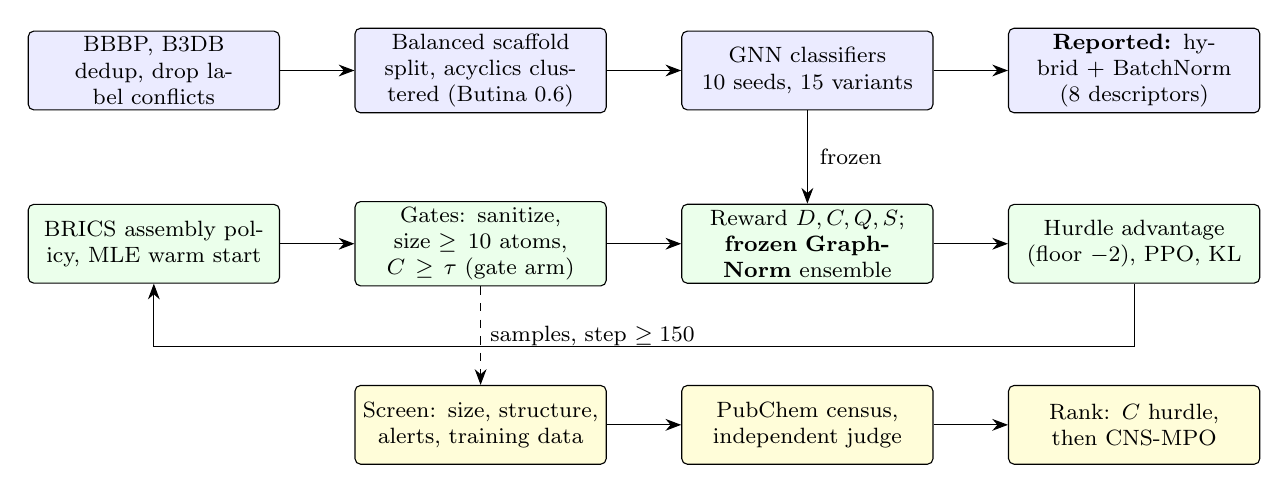
\begin{tikzpicture}[
  box/.style={draw,rounded corners=2pt,align=center,font=\footnotesize,minimum height=10mm,text width=3.05cm,fill=white,inner sep=2pt},
  clf/.style={box,fill=blue!8}, gen/.style={box,fill=green!8}, scr/.style={box,fill=yellow!15},
  arr/.style={-{Stealth[length=2mm]},thin}]
\node[clf] (data) at (0,0) {BBBP, B3DB\\dedup, drop label conflicts};
\node[clf] (split) at (4.15,0) {Balanced scaffold split, acyclics clustered (Butina 0.6)};
\node[clf] (clf) at (8.3,0) {GNN classifiers\\10 seeds, 15 variants};
\node[clf] (rep) at (12.45,0) {\textbf{Reported:} hybrid + BatchNorm (8 descriptors)};
\node[gen] (pol) at (0,-2.2) {BRICS assembly policy, MLE warm start};
\node[gen] (gate) at (4.15,-2.2) {Gates: sanitize, size $\ge10$ atoms, $C\ge\tau$ (gate arm)};
\node[gen] (rew) at (8.3,-2.2) {Reward $D,C,Q,S$; \textbf{frozen GraphNorm} ensemble};
\node[gen] (adv) at (12.45,-2.2) {Hurdle advantage (floor $-2$), PPO, KL};
\node[scr] (scr) at (4.15,-4.5) {Screen: size, structure, alerts, training data};
\node[scr] (cen) at (8.3,-4.5) {PubChem census, independent judge};
\node[scr] (rank) at (12.45,-4.5) {Rank: $C$ hurdle, then CNS-MPO};
\draw[arr](data)--(split);\draw[arr](split)--(clf);\draw[arr](clf)--(rep);
\draw[arr](clf)--node[right,font=\footnotesize,xshift=1pt]{frozen}(rew);
\draw[arr](pol)--(gate);\draw[arr](gate)--(rew);\draw[arr](rew)--(adv);
\draw[arr](adv.south)--++(0,-0.8)-|(pol.south);
\draw[arr,dashed](gate.south)--node[right,font=\footnotesize]{samples, step $\ge150$}(scr);
\draw[arr](scr)--(cen);\draw[arr](cen)--(rank);
\end{tikzpicture}}
\caption{Pipeline. Blue: classifier stage (trained twice, because it has two incompatible roles). Green: generator loop; the gates and the floor act \emph{outside} the standardized advantage. Yellow: screening and evaluation of the pooled output.}
\label{fig:pipeline}
\end{figure}

\paragraph{Data and split.} BBBP \cite{martins2012} and B3DB \cite{meng2021} are trained and evaluated independently, because B3DB aggregates BBBP. Two external holdouts, Adenot \cite{adenot2004} (59 molecules) and Wang \cite{wang2018} (55), are filtered to be scaffold-disjoint from both training sets; the leak filter removes about $96.5\%$ of each source. The split is a balanced Bemis--Murcko scaffold split with per-seed shuffling (the size-sorted DeepChem variant leaves validation and test $100\%$ positive on BBBP, so ROC-AUC is undefined). \emph{Acyclic molecules have an empty Murcko scaffold and had collapsed into one group that always landed in train: 95 of 1{,}965 BBBP and 311 of 7{,}805 B3DB molecules were never tested.} They are now grouped by Morgan/Tanimoto similarity (Butina \cite{butina1999}, cutoff 0.6). This costs about $0.037$ ROC-AUC on BBBP; our earlier figures were optimistic, not wrong by accident. Each seed is a different split, so every $\pm$ includes split variance.

\paragraph{Classifier.} One skeleton (three blocks of convolution, normalization, ReLU and dropout $0.3$, width $128$; mean$\|$max atom readout; two-layer head) with GCN, GraphSAGE, GIN, GAT, bond-aware GINE/GAT-E/SAGE-E, and the hybrid that appends 8 RDKit descriptors (including a CNS-MPO proxy) to the graph embedding. A LightGBM model on the same descriptors and folds is the baseline.

\paragraph{Two classifier roles.} The classifier is trained twice. The \emph{reported} model uses BatchNorm (best scores). The \emph{frozen reward} uses GraphNorm: in training mode BatchNorm makes a molecule's logit depend on which other molecules share its batch (drift $3.97\times10^{-2}$, versus $6\times10^{-8}$ for GraphNorm \cite{cai2021}), so the reward would stop being a function of the molecule. The reward ensemble is GIN/GAT/GINE at seed 0, without descriptors; every load verifies feature hash, fold identity and norm identity.

\paragraph{Generator.} The settled generator assembles BRICS fragments \cite{degen2008}; it reconstructs $2039/2039$ BBBP molecules exactly and is valid by construction up to aromaticity ($95.4\%$ sanitization untrained, $0.9996$ after the MLE warm start). A SELFIES GRU \cite{krenn2020} is kept as a comparison. A maximum-likelihood warm start is mandatory: from a uniform policy every group is invalid, the group standard deviation is zero and GRPO receives no gradient. Group size $N=64$, $K=4$ PPO epochs with clip $0.2$, Adam at $10^{-4}$, two discriminator steps per generator step (after the PPO block, so each group's advantages use one fixed discriminator), settled point $\mathrm{KL}=1.0$ and $250$ steps. The reward is a weighted sum of the discriminator $D$, the classifier $C$, QED $Q$ \cite{bickerton2012} and $S=(10-\mathrm{SA})/9$ \cite{ertl2009}, with $D$ and $C$ weights annealed linearly over 100 steps ($D$: $1.0\to0.3$; $C$: $0.2\to1.5$; $Q,S$: $0.5$).

\section{What a Group-Standardized Update Can See}\label{sec:theory}
Let $r\in\R^N$ be group rewards with validity indicator $v$, $n$ valid and $k=N-n$ invalid molecules. The \emph{pooled} advantage is $A_i=(r_i-\bar r)/s(r)$. Invalid molecules receive a flat reward far below the valid cluster, so they dominate the pooled standard deviation.

\begin{proposition}[Spread under pooling]\label{prop:spread}
If the $n$ valid rewards have mean $\mu_v$ and variance $\sigma_v^2$, and invalid ones receive $r_0$ with $\Delta=\mu_v-r_0$, then the standard deviation of the pooled advantages among valid molecules is
\[
\rho=\Big(\tfrac{(N-1)\sigma_v^2}{(n-1)\sigma_v^2+nk\Delta^2/N}\Big)^{1/2}\ \to 0 \text{ as } |\Delta|/\sigma_v\to\infty .
\]
\end{proposition}
Measured on BBBP groups an invalid molecule sits $\Delta\approx8.5\,\sigma_v$ below the valid cluster, so one invalid molecule in 64 costs $31\%$ of the ranking scale and three cost $51\%$ (Table~\ref{tab:spread}). Standardization is affine, so \emph{order} is preserved ($\operatorname{corr}(A,C)$ is unchanged); what is lost is scale. The \emph{hurdle} estimator standardizes among valid molecules only and assigns invalid ones a fixed floor $f$; its spread is $1$ for every $k$, and the net push on invalid sequences is $kf<0$ rather than zero-sum. This analysis was run on static groups sampled from the warm start; the hurdle estimator is used in all training runs, so the pooled estimator was never trained against.

\begin{table}[t]
\centering
\caption{Ranking spread among valid molecules, $N=64$. Prediction uses $\Delta=8.5\sigma_v$; ``logged'' is the repository's resampling experiment. The hurdle estimator gives $1.00$ for every $k$.}
\label{tab:spread}
\begin{tabular}{@{}lcccc@{}}\toprule
invalid molecules $k$ & 0 & 1 & 2 & 3\\\midrule
predicted $\rho$ & 1.00 & 0.69 & 0.56 & 0.49\\
logged $\rho$ (pooled) & 1.00 & 0.70 & 0.60 & 0.49\\\bottomrule
\end{tabular}
\end{table}

\begin{lemma}[Blindness to absolute level]\label{lem:blind}
For $a>0$, $A(a\,r+b\mathbf 1)=A(r)$ for both estimators. Hence, without the KL term, the update depends on rewards only through $A$: two groups that differ by a positive affine map (including one uniformly worse by a constant) produce the same update.
\end{lemma}
Consequently a reward term that is constant over the group does nothing, however large, and a term's influence is governed by $w_j\sigma_j$, the weight times its within-group spread. If terms are uncorrelated within the group, $\operatorname{corr}(A,T_j)=w_j\sigma_j/(\sum_k w_k^2\sigma_k^2)^{1/2}$; the logged mean pairwise term correlation is $+0.009$ (discriminator vs.\ classifier $-0.258$), so this is a first-order guide. What can restrain the policy \emph{absolutely} is what enters outside $A$: the validity/size gate (through the floor) and the KL penalty. A term that varies within the group restrains only relatively. A saturating classifier illustrates the consequence: if $C=\sigma(\ell)$ with $\ell$ spread $s$ around mean $\mu$, then $\sd(C)\approx s\,\sigma'(\mu)\sim s\,e^{-\mu}$, so a linearly annealed weight cannot keep $w_C\sd(C)$ constant as the group moves up the logit scale.

\section{Experiments}
\subsection{The classifier}\label{sec:clf}
\begin{table}[t]
\centering
\caption{Test ROC-AUC (mean $\pm$ sd over 10 seeds; each seed a different scaffold split). Wang is the informative external holdout ($n=55$); Adenot ($n=59$) is saturated near $0.99$ for every family. Per-model values are in Supplement Table~S1.}
\label{tab:auc}
\begin{tabular}{@{}lccc@{}}\toprule
family (best member) & BBBP & B3DB & Wang\\\midrule
LightGBM, 8 descriptors & $0.881\pm0.039$ & $0.852\pm0.040$ & --\\
base GNN & $0.895\pm0.038$ (GCN) & $0.893\pm0.051$ (SAGE) & $0.846$\\
edge-aware & $0.893\pm0.031$ & $0.889\pm0.052$ & $0.853$\\
hybrid, GraphNorm (\emph{frozen reward}) & $0.909\pm0.029$ (GAT) & $0.900\pm0.052$ (SAGE) & $0.839$\\
hybrid, BatchNorm (\emph{reported}) & $\mathbf{0.921\pm0.032}$ (GCN) & $\mathbf{0.905\pm0.047}$ (GIN) & $0.850$\\\bottomrule
\end{tabular}
\end{table}
Table~\ref{tab:auc} and Figure~\ref{fig:clf} show the picture. Absolute numbers are not comparable to the $0.65$--$0.70$ BBBP scaffold figures in the literature, which come from the degenerate size-sorted protocol. Four findings stand.
\begin{enumerate}[leftmargin=*,itemsep=1pt]
\item \textbf{Operator choice is not resolved.} At ten seeds, 4 of 24 within-family pairs (base and hybrid-BatchNorm families, both datasets) separate at $95\%$, and 13 of 55 across all models; every surviving effect is $0.004$--$0.02$. A three-seed claim that GAT beat GIN by $1.4$ paired standard deviations did not replicate ($+0.0109$, CI $[-0.0057,+0.0275]$).
\item \textbf{Two components help, and they stack} (Figure~\ref{fig:comp}): 8 descriptors ($+0.0099$, SEM $0.0019$) and BatchNorm over GraphNorm ($+0.0074$, SEM $0.0023$); together $+0.0195\pm0.0024$ against $+0.0173$ if independent (full table: Supplement Table~S2). Everything adding structural reasoning (recurrence, motif graphs replacing atoms, long-range connectivity) is neutral or harmful. A plausible reading is that BBB permeability behaves like a property of bulk composition rather than long-range topology; we did not test this mechanism directly.
\item \textbf{In-distribution rank does not predict transfer.} Across the 11 GraphNorm-family models the correlation between BBBP and Wang AUC is $r=-0.45$ ($p=0.16$): suggestive, not established, but there is no evidence \emph{for} transfer. The plain hybrid ranks 1st--3rd in-distribution and 7th--9th on Wang. BatchNorm's gain ($+0.0101$ in distribution, $+0.0108$ on Wang) is the one effect that keeps its sign and size. With $n=55$ the per-model sd across seeds on Wang is about $0.05$, larger than the span between families ($0.014$), so no family is separated there.
\item \textbf{The score ranks well and calibrates poorly.} On pooled hybrid-GraphNorm test folds ($n=1970$) the Brier score is $0.103$ and ECE $0.074$; the model is underconfident in every bin (a score of $0.25$ is permeable $60\%$ of the time; Supplement Table~S3) but the mapping is monotone, so ranking, and therefore the group-standardized update, is unaffected. On Wang ECE is $0.094$ with $4$--$7$ molecules per bin, too few to characterize its shape.
\end{enumerate}

\begin{figure}[t]\centering
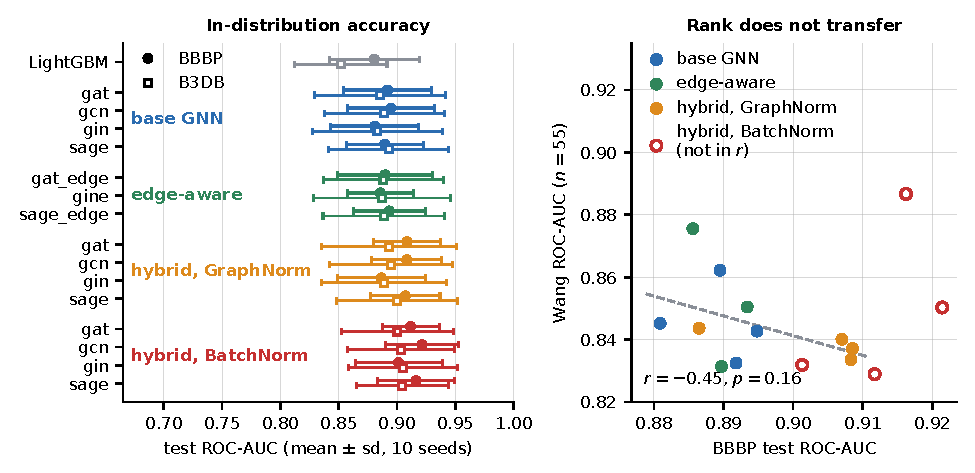
\includegraphics[width=\linewidth]{figs/classifier.pdf}
\caption{Left: ROC-AUC per model (points) and per-model sd over seeds (bars); the ranges overlap heavily. Right: in-distribution versus external-holdout AUC for the 11 GraphNorm-family models; hybrid-BatchNorm models (hollow) are shown but excluded from $r$.}
\label{fig:clf}
\end{figure}
\begin{figure}[t]\centering
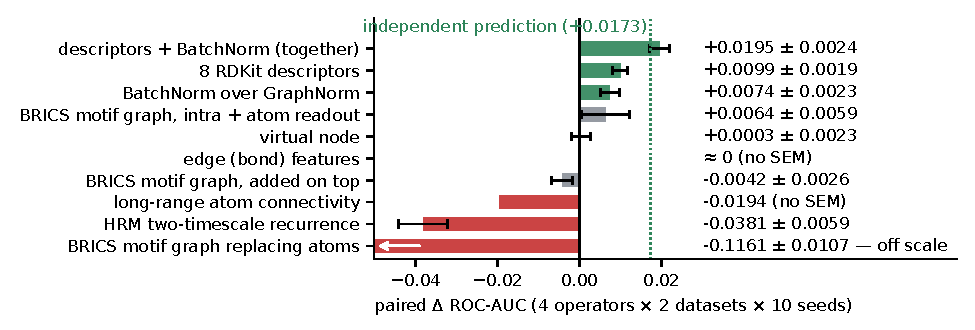
\includegraphics[width=\linewidth]{figs/components.pdf}
\caption{Paired effect of each component on ROC-AUC (pooled over four operators, two datasets, ten seeds; bars are SEM where reported; values from the repository's component table). The wide mean$\|$max atom readout ($+0.130$), part of every model's skeleton, is omitted.}
\label{fig:comp}
\end{figure}

\subsection{An unconstrained loop collapses while every logged metric looks healthy}\label{sec:collapse}
The baseline (SELFIES policy, $\mathrm{KL}=0.02$, no size gate, 200 steps, three seeds) climbs in reward while destroying structure (Table~\ref{tab:collapse}, Figure~\ref{fig:collapse}). Validity \emph{rises}. The original logging (validity, mean reward, distinct-SMILES fraction) was blind: scaffold fraction falls $20\%$ below its opening level at steps 24, 15 and 12, while distinct SMILES does so only at steps 112, 169 and 144, a lead of $88$--$154$ steps. Seeds are not interchangeable: seed 0 collapses much earlier and harder (scaffold fraction $0.17$ at step 90 against $0.75$ and $0.73$).

\begin{table}[t]
\centering
\caption{Unconstrained baseline, three seeds; range over seeds.}
\label{tab:collapse}
\begin{tabular}{@{}lcc@{}}\toprule
quantity & first 10 steps & last 10 steps\\\midrule
scaffold fraction & 0.72 to 0.80 & 0.07 to 0.14\\
Tanimoto distance & 0.90 to 0.91 & 0.25 to 0.45\\
TPSA spread ratio & 0.41 to 0.48 & 0.12 to 0.18\\
classifier term $C$ (mean) & 0.87 to 0.88 & 0.98 to 0.99\\
valid fraction & 0.98 to 0.99 & 1.00\\\bottomrule
\end{tabular}
\end{table}
\begin{figure}[t]\centering
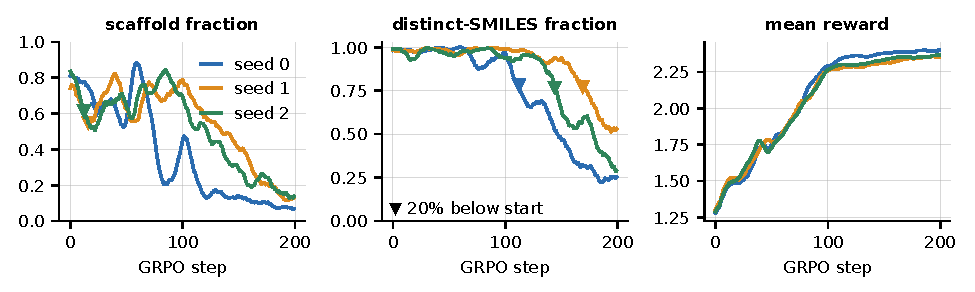
\includegraphics[width=\linewidth]{figs/collapse.pdf}
\caption{Unconstrained SELFIES baseline, three seeds, 9-step smoothing (each step is one group of 64). Structure collapses and string-level uniqueness lags it; the reward rises throughout.}
\label{fig:collapse}
\end{figure}

\paragraph{Not all of it is reinforcement learning.} The MLE warm start is already $0.72\times$--$0.87\times$ as dispersed as BBBP on four descriptors; GRPO accounts for $58\%$--$71\%$ of the loss of spread. Structurally the warm start matches BBBP (scaffold fraction $0.750\pm0.026$ vs.\ $0.765\pm0.021$), so all structural collapse is GRPO's. This bounds what a KL fix can recover, since the KL anchor \emph{is} the warm start.

\paragraph{The classifier term goes uninformative.} In seed 0 the within-group standard deviation of $C$ falls from $0.173$ at step 0 to $0.004$--$0.006$ at steps 150--199, with $100\%$ of molecules above $0.95$. By Lemma~\ref{lem:blind} the weight $w_C$ rising $7.5\times$ cannot compensate. In logit space the between-molecule signal falls from $2.26$ to $0.41$ while the classifier's own MC-dropout noise stays near $0.95$, so signal-to-noise crosses $1$ between steps 100 and 150 and the term ranks little beyond noise. We caution that $w_C\sd(C)$ is only a first-order measure of influence (it ignores the other terms' spreads), and that the logit-scale spread itself fell, so saturation and diversity collapse are entangled.

\subsection{Which anchors work}\label{sec:anchors}
A KL sweep (SELFIES, seed 0, 120 steps; Table~\ref{tab:kl}) passes our retention criterion (scaffold fraction $\ge0.70\times$ and $\sd C\ge0.50\times$ the warm start's, with mean $C$ above it by $>0.01$) only at $\beta\in\{0.3,1.0\}$, and the price is the reward gain shrinking from $0.082$ to $0.043$: the anchor works largely by keeping the policy near its start. The criterion tracks $\sd C$ because one on mean $C$ alone is satisfied by the failure. The size gate ($\ge10$ heavy atoms) at $\beta=0.3$, three seeds, raises scaffold fraction $0.769\pm0.027\to0.828\pm0.004$ and cuts undersized molecules from $10.4\%$ to $2.1\%$ at a cost of $0.004$ in mean $C$; note this is measured on top of a KL that already prevents collapse. Reweighting inside the advantage did not help: a logit transform of $C$ \emph{worsened} the collapse (scaffold fraction $0.741\to0.349$, one seed), and in that arm the policy converged on carbon tetrachloride and freon-12 (CCl$_4$ scores $2.280$ against caffeine's $2.063$). This is not an extrapolation error: of 65 BBBP molecules with at most 8 heavy atoms, 62 are positive, including chloroform and nitrous oxide, which do cross the barrier. The floor $f=-2$ was swept (single seed): $-1.0$ measurably hurts (scaffold $0.834$ vs.\ $0.887$; undersized molecules more than double), while $-4.0$ changes nothing (scaffold $0.881$); $-2$ is the knee.

\begin{table}[t]
\centering
\caption{KL sweep, SELFIES, seed 0, 120 steps (single seed). Warm start: scaffold fraction $0.736$, $\sd C=0.175$, mean $C=0.835$. A setting passes if scaffold fraction $\ge0.70\times$ and $\sd C\ge0.50\times$ the warm start's, and mean $C$ exceeds it by $>0.01$.}
\label{tab:kl}
\begin{tabular}{@{}lcccccc@{}}\toprule
$\beta$ & scaffold & Tanimoto & mean $C$ & $\sd C$ & gain in $C$ & passes\\\midrule
0.02 & 0.175 & 0.683 & 0.976 & 0.017 & 0.147 & no\\
0.1 & 0.638 & 0.854 & 0.951 & 0.060 & 0.115 & no\\
0.3 & 0.777 & 0.897 & 0.920 & 0.099 & 0.082 & yes\\
1.0 & 0.763 & 0.914 & 0.887 & 0.147 & 0.043 & yes\\\bottomrule
\end{tabular}
\end{table}

\begin{figure}[t]\centering
\begin{minipage}[t]{.49\linewidth}\centering
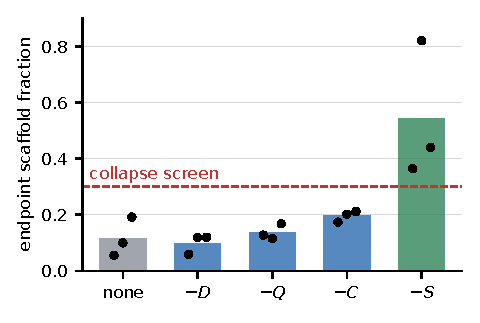
\includegraphics[width=\linewidth]{figs/ablation.pdf}
\caption{Term ablation: endpoint scaffold fraction when a term is dropped (3 seeds; bar = mean).}\label{fig:abl}
\end{minipage}\hfill
\begin{minipage}[t]{.49\linewidth}\centering
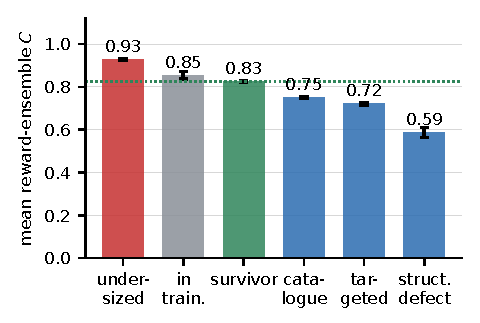
\includegraphics[width=\linewidth]{figs/rejected.pdf}
\caption{Mean $C$ by screening verdict (gate arm, $n=33{,}227$). Undersized molecules score highest.}\label{fig:rej}
\end{minipage}
\end{figure}

\paragraph{Term ablation.} Dropping the synthesizability term $S$ is the only change after which no seed collapses (scaffold fraction $+0.426$, 3/3 seeds, 0/3 still collapsed; Figure~\ref{fig:abl}). Dropping $C$ helps by about a fifth as much ($+0.080$) and all three seeds still collapse; QED and $D$ do little ($+0.021$, $-0.016$). Zeroing a term is not its marginal contribution (standardization rescales what remains), the arms are not weight-matched, $n=3$, and the $0.30$ collapse screen is arbitrary. With $w_C=0$, mean $C$ still reaches $0.786$ against $0.745$ for real BBBP molecules: permeability is largely a side effect of what $Q$, $S$ and $D$ select for. Dropping $S$ has not been shown to be safe, only to restore diversity; final samples have mean SA $2.9$--$3.3$ against $3.05$ for real BBB-positive molecules.

\subsection{BRICS assembly, and a retraction}\label{sec:brics}
An earlier version of our analysis reported that BRICS loses $0.27$ of scaffold diversity and attributed it to the compact action space. \emph{That explanation is retracted.} The measurement was real but taken at $\mathrm{KL}=0.3$, a value validated for SELFIES that does not transfer: the same coefficient yields $10.7\times$ the KL on BRICS (about 5.1 decisions over a 6051-way softmax against about 38.6 over 77 tokens, under a token-level masked mean). At $\mathrm{KL}=0.3$ BRICS reaches scaffold $0.643$ and uniqueness $0.744$; raising the coefficient to $1.0$ gives $0.864$ and $0.982$, i.e.\ $+0.221$ scaffold and $+0.238$ uniqueness (paired $p\le0.005$; Table~\ref{tab:brics}). Properly compared as frontiers, the two families interleave where they overlap, BRICS dominates on validity and extends further (scaffold $0.906$ vs.\ $0.835$), and it costs a sweep SELFIES does not. BRICS also tracks real drugs on an instrument gap, $C_{\text{reward}}-C_{\text{unused B3DB judge}}$ ($+0.0381$ vs.\ $+0.0373$ for real drugs and $+0.0551$ for SELFIES; Welch $p=0.003$, $n=12$ per arm, per-sample ranges overlap). At the settled point over ten policy seeds, scaffold fraction is $0.854\pm0.006$ (SEM), exact-duplicate freedom $0.982$, and sanitization $0.9996$. (Three seeds had read $0.864$: one unlucky draw on the one axis with a large spread.) Aromaticity is not guaranteed by construction, and part of what the warm start teaches is toolkit avoidance rather than chemistry.

\begin{table}[t]
\centering
\caption{BRICS versus SELFIES at steps 225--250, mean over four cells (reward seed $\times$ warm start). Warm-start reference at the same $n=64$: scaffold $0.854$, unique $0.990$.}
\label{tab:brics}
\begin{tabular}{@{}lccccc@{}}\toprule
arm & scaffold & unique & $C$ & reward & sanit.\\\midrule
BRICS, KL 0.3 (inherited) & 0.643 & 0.744 & 0.932 & 2.280 & 0.9998\\
\textbf{BRICS, KL 1.0 (tuned)} & \textbf{0.864} & \textbf{0.982} & 0.847 & 2.090 & 0.9998\\
SELFIES, KL 0.3 (validated) & 0.821 & 0.995 & 0.900 & 2.080 & 0.9946\\\bottomrule
\end{tabular}
\end{table}

\subsection{Permeability as a gate}\label{sec:gate}
Because the reward is a weighted sum, a monotone $C$ term pays the policy to \emph{climb} toward whatever maximizes $C$. The \textsc{gate} arm drops the $C$ term and instead requires $C\ge\tau$, with $\tau=0.615$ the 5th percentile of real BBB-positive molecules under the ensemble (calibrated on the positive class, never on generated output).

\begin{table}[t]
\centering
\caption{Arm A ($C$ as a term) versus the gate arm; ten policy seeds, BBBP.}
\label{tab:gate}
\begin{tabular}{@{}lcc@{}}\toprule
& A: $C$ as term & \textsc{gate}\\\midrule
pooled distinct molecules & 19{,}219 & \textbf{33{,}227} (+73\%)\\
survivors of the screen & 6{,}591 & \textbf{11{,}329} (+72\%)\\
survival rate & 34\% & 34\%\\
training molecules reproduced & 1{,}747 (88.9\%) & \textbf{1{,}345 (68.4\%)}\\
novel, whole pool & 72.0\% & 79.4\%\\
survivor $C$ & 0.854 & 0.826\\\bottomrule
\end{tabular}
\end{table}
\begin{figure}[t]\centering
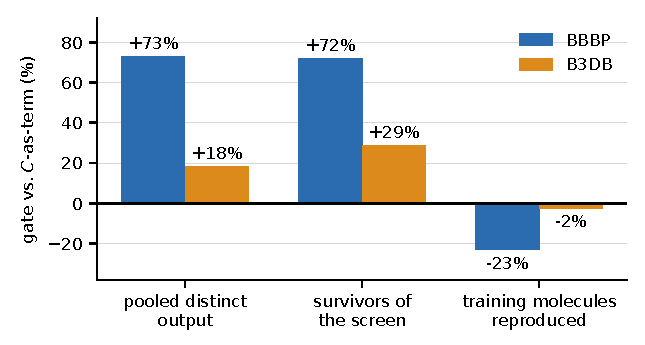
\includegraphics[width=.66\linewidth]{figs/gate.pdf}
\caption{The gate's benefit on two corpora (changes relative to arm A; B3DB gate recalibrated to its own real-positive 5th percentile, $\tau=0.476$). The benefit shrinks about fourfold where the corpus is large.}
\label{fig:gate}
\end{figure}
Two apparent changes are not results: the in-training valid fraction falls ($0.979\to0.854$) while RDKit sanitization is unchanged, because gated molecules count as invalid; and in-training mean $C$ rises purely because the gate truncates its low tail. Within-group scaffold diversity falls $0.851\to0.820$ ($p=0.19$) while pooled distinct output rises, two different statistics. \textbf{The gate does nothing about the objective}: CCl$_4$ scores $C=0.987$ and passes any threshold calibrated on real BBB-positive drugs; the size gate remains the only thing that blocks tiny solvents. Scoring the 45{,}701 pooled molecules that the screen rejected makes this concrete (Figure~\ref{fig:rej}): undersized molecules (about 8 heavy atoms) have the highest mean $C$ in the pool ($0.928$, identical across three arms), while every other rejection reason scores lower than survivors ($0.826$): catalogue alerts $0.750$, targeted alerts $0.721$, structural defects $0.586$. The size gate is load-bearing; the alert screens are complementary rather than counterweights.

\paragraph{Replication on B3DB.} On B3DB (30 runs, 7{,}805 molecules) the classifier-swap null holds (below), but the gate claim shrinks to $+18\%$ pooled distinct output and $+29\%$ survivors, with reproduction of training molecules $-23\%\to-2\%$ and corpus coverage $46.1\%\to45.0\%$ (Figure~\ref{fig:gate}). The proposed mechanism is that the gate's benefit scales with how badly the policy had memorized its corpus: on BBBP it had regenerated $88.9\%$ of 1{,}965 molecules, whereas a 7{,}805-molecule corpus is only $46\%$ covered anyway. The revised claim is that a hurdle helps most where the corpus is small enough to memorize. The census and cross-reward matrix have not been run on B3DB.

\subsection{Does GRPO beat its own warm start?}
\begin{table}[t]
\centering
\caption{One matched draw of 8 groups of 64 per arm. Random assembly over the same vocabulary produces giant chains, so its high scaffold fraction is an artefact.}
\label{tab:base}
\setlength{\tabcolsep}{3pt}
\begin{tabular}{@{}lccccccc@{}}\toprule
arm & valid & $C$ & QED & MPO & scaff. & uniq. & heavy\\\midrule
random policy & 0.943 & 0.519 & 0.293 & 0.345 & 0.961 & 0.998 & 167.4\\
MLE warm start & 1.000 & 0.739 & 0.605 & 0.714 & 0.857 & 0.992 & 24.6\\
GRPO (arm A) & 1.000 & 0.878 & 0.680 & 0.741 & 0.855 & 0.986 & 22.8\\
GRPO (gate arm) & 1.000 & 0.820 & 0.680 & 0.747 & 0.855 & 0.941 & 22.6\\
real BBBP control & 1.000 & 0.763 & 0.623 & 0.713 & 0.844 & 1.000 & 24.4\\\bottomrule
\end{tabular}
\end{table}
\begin{figure}[t]\centering
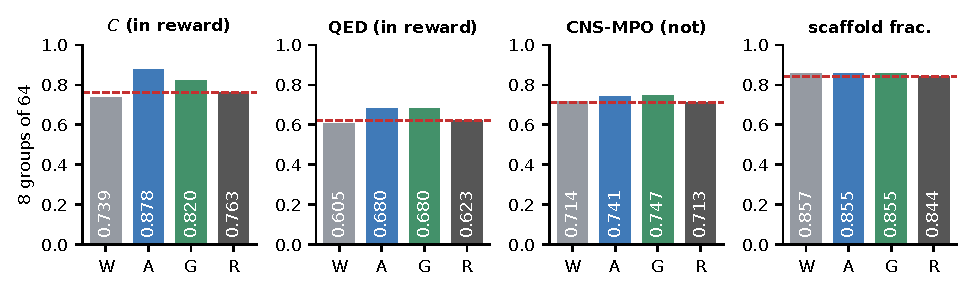
\includegraphics[width=\linewidth]{figs/baselines.pdf}
\caption{Draw of Table~\ref{tab:base} (matched $n=64$); W: warm start, A: GRPO arm A, G: GRPO gate arm, R: real BBBP (dashed). Gains land on terms in the reward ($C$, QED), not on CNS-MPO.}
\label{fig:base}
\end{figure}
The warm start already sits at real-BBBP level on QED ($0.605$ vs.\ $0.623$), CNS-MPO ($0.714$ vs.\ $0.713$) and scaffold fraction ($0.857$ vs.\ $0.844$) before any reinforcement learning. Welch tests at 16 groups per arm against the warm start: arm A gains on $C$ ($+0.126$, $d=3.53$) and QED ($+0.054$, $d=1.90$), both $p<10^{-4}$, but not on CNS-MPO ($+0.008$, $d=0.27$, $p=0.45$). The gate arm's scaffold gain ($+0.043$, $d=1.09$, $p=0.005$) and uniqueness cost ($-0.023$, $d=1.35$, $p=0.001$) are less robust than these: the single 8-group draw in Table~\ref{tab:base} shows neither (scaffold $0.855$ vs.\ $0.857$; uniqueness $0.941$ vs.\ $0.992$), so draw-to-draw variation is of the order of the effect and we treat the diversity claim as tentative. GRPO earns its place, but it delivers higher reward, not better molecules by an independent measure. No REINVENT or MOSES comparison is made: this generator trains on 1{,}965 BBBP molecules rather than ZINC or ChEMBL, so such a comparison would answer a different question.

\subsection{Is the generator hacking its judge?}
\paragraph{Swapping the reward classifier changes nothing.} A second arm trains against the reported hybrid-BatchNorm classifier instead (ten seeds, paired). Scaffold diversity ($+0.0025$, $p=0.73$), validity ($p=0.94$) and uniqueness ($p=0.65$) do not separate; only Tanimoto distance does ($p=0.007$, a $0.2\%$ relative effect). Provenance is near-identical ($9.1\%$ vs.\ $8.7\%$ in training data; $72.0\%$ vs.\ $72.2\%$ novel). In a $2\times2$ of trained-on versus scored-by reward (Table~\ref{tab:cross}), in-loop advantage is $+0.010$ and $+0.007$: each arm scores almost as well under the reward it never saw, and the two rewards correlate at Spearman $+0.71$. On the B3DB replication the paired swap again shows no effect (scaffold $p=0.79$, validity $0.42$, Tanimoto $0.45$; uniqueness $p=0.04$ fails Bonferroni over four tests). Predictor accuracy still does not transfer to generator behaviour, now on two datasets.

\begin{table}[t]
\centering
\caption{Trained-on versus scored-by reward, each cell as a fraction of that reward's own real-BBB-positive control. Bold: in-loop. Real-molecule controls (raw $C$) are in the last two rows.}
\label{tab:cross}
\begin{tabular}{@{}lcc@{}}\toprule
& scored by ensemble & scored by hybrid-BatchNorm\\\midrule
A: trained on ensemble & \textbf{0.941} & 0.929\\
B: trained on hybrid-BatchNorm & 0.931 & \textbf{0.936}\\
real BBB-positive (raw $C$) & 0.908 & 0.866\\
real BBB-negative (raw $C$) & 0.263 & 0.167\\\bottomrule
\end{tabular}
\end{table}
\paragraph{Out-of-loop judge.} The reported classifier (descriptors the reward model never sees, a different norm, ten splits) scores the arm-A survivors at $0.825\pm0.219$ ($88.9\%$ above $0.5$) against $0.889\pm0.175$ for real BBB-positive and $0.197\pm0.187$ for real BBB-negative molecules: mean optimism $+0.029$, and over the 250 top-ranked survivors the gap is $+0.008$ with no molecule above $0.3$. This rules out \emph{ensemble-specific} hacking. It does not touch the objective problem: the independent judge scores CCl$_4$ at $1.000$, above caffeine's $0.976$, because two models trained on BBBP agree that solvents cross membranes, as they do.

\subsection{What the output looks like}
\paragraph{Provenance.} All 19{,}219 pooled arm-A molecules were resolved against PubChem's full CID-to-InChIKey table (124.7M compounds, matched on the full InChIKey): $9.1\%$ are in the training data, $18.9\%$ exist but were never seen, and $72.0\%\pm0.6\%$ have no record. Among survivors, $31.4\%$ are known and $68.6\%$ novel. Output-level memorization is therefore low, although those 1{,}747 distinct training molecules are $88.9\%$ of the corpus: the policy regenerates most of its corpus, but most of what it emits is new. The novel figure is an upper bound (tautomers are not normalized), means absence from PubChem and the corpus only, and is not a quality signal. An independent 200-molecule sample predicted $7.5/20.0/72.5\%$ before the census ran.

\paragraph{Survivors.} The 11{,}329 gate-arm survivors form 7{,}543 Butina clusters (largest 25): there are no large families, and 16 motifs that none of the screened catalogues encode (peroxides, azo, isocyanate, thiol, P, B, Si, Se/Te and others) match $0$ of $11{,}329$. But $27.1\%$ are physicochemically unable to cross, and the classifier rewards the lipophilic ones ($\log P>5$: $15.8\%$, mean $C=0.837$) while correctly penalizing polarity, size and donor count. Scaffold novelty is reported, not enforced: $23.5\%$ of gate-arm survivors with a ring system share an exact Murcko scaffold with BBBP ($34.8\%$ for arm A). One survivor is constitutionally identical to LSD; it is absent from BBBP even after flattening, so it is not a leak, but it is a demonstration of the objective working as specified, not a novelty or safety signal.

\paragraph{Ranking is a separate defect.} Ranking the shortlist by absolute $C$ selects the greasy extreme (Table~\ref{tab:rank}); the gate arm shows the same drift ($+2.02$ log\,$P$) despite never optimizing $C$, so this is a ranking defect rather than a reward defect. We therefore rank by CNS-MPO \cite{wager2010} behind the permeability hurdle $C\ge0.615$. CNS-MPO saturates too ($950$ of $9{,}722$ survivors clearing the hurdle score a perfect $1.000$), so ties are broken by $C$. The shortlist (Figure~\ref{fig:mols}) keeps $C$ at $0.988$ while moving MPO from $0.487$ to $1.000$. CNS-MPO is a desirability composite, not a measurement: the shortlist is \emph{more} idealized than real CNS drugs (log\,$P$ $1.24$ against $2.67$).

\begin{table}[t]
\centering
\caption{Three selections from the 11{,}329 gate-arm survivors.}
\label{tab:rank}
\begin{tabular}{@{}lccccc@{}}\toprule
& log\,$P$ & TPSA & QED & MPO & $C$\\\midrule
all survivors & 3.12 & 50.1 & 0.68 & 0.714 & 0.826\\
top 25 by $C$ (old) & 5.15 & 18.9 & 0.64 & 0.487 & 0.997\\
top 25 by MPO behind $C\ge0.615$ (new) & 1.24 & 52.3 & 0.79 & 1.000 & 0.988\\
real BBB-positive drugs & 2.67 & 54.1 & 0.67 & 0.753 & --\\\bottomrule
\end{tabular}
\end{table}
\begin{figure}[t]\centering
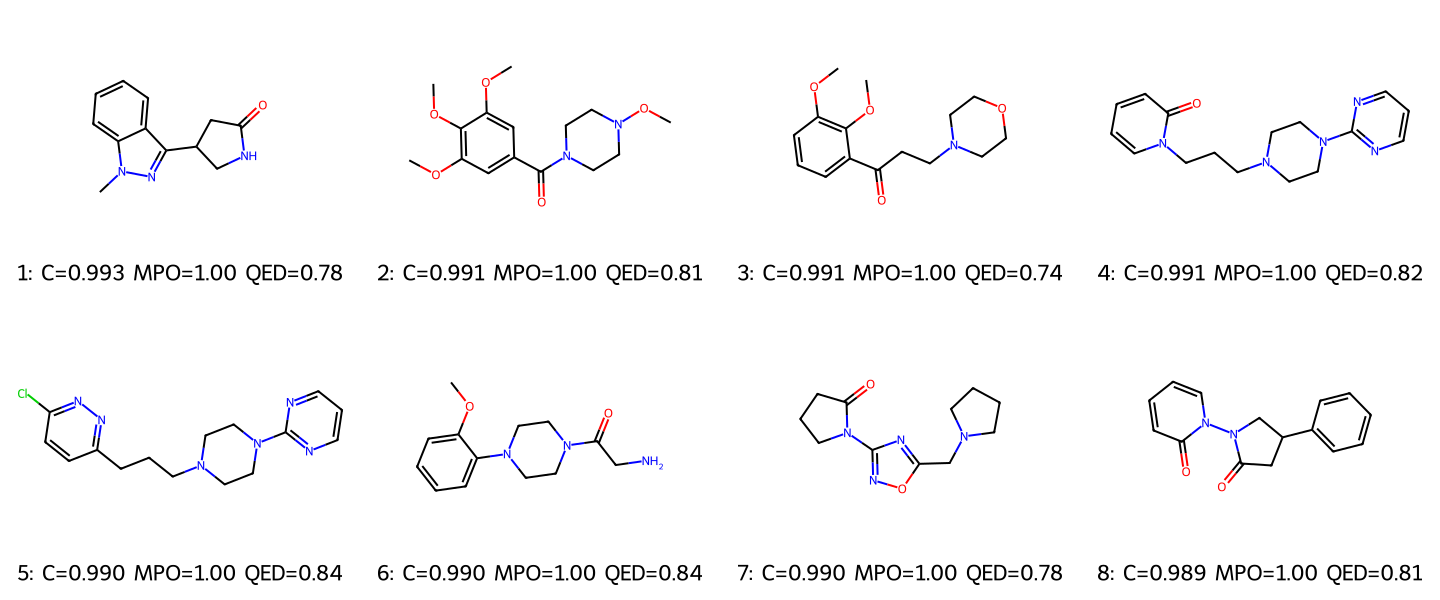
\includegraphics[width=.8\linewidth]{figs/shortlist.png}
\caption{First 12 of the CNS-MPO-ranked shortlist (gate arm); labels give reward-ensemble $C$, CNS-MPO and QED. Hypotheses only.}
\label{fig:mols}
\end{figure}

\subsection{Rank-based reduction}
The reward is a linear scalarization, so no weighting reaches a concave fold of the Pareto front \cite{das1997}; on sampled groups, 2000 random weightings reach $0.48$ of the per-group front (the probe script is not in the repository, so the figure is indicative). A dominance-and-crowding reduction \cite{deb2002}, computed once per group, was compared with the linear sum (SELFIES, $\mathrm{KL}=0.3$, 200 steps, four seeds, paired; Supplement Table~S8). Property spread improved on all four seeds (TPSA $0.410\to0.524$, log\,$P$ $0.683\to0.784$, MW $0.481\to0.585$), but at a cost in $C$ ($0.925\to0.891$, worse on 4/4 seeds), no scaffold improvement ($0.811\to0.780$) and a slightly worse instrument gap ($+0.036\to+0.042$, worse on 3/4 seeds). Because this arm also moved less, the coverage gain may partly reflect weaker optimization pressure. It was not promoted to the default.

\section{Practical Guidance}
Five practices follow from the measurements. (i) \emph{Log structure, not strings:} scaffold fraction led distinct-SMILES by $88$--$154$ steps. (ii) \emph{Put every hard constraint outside the standardized advantage} (a size gate, an invalidity floor, a KL penalty); inside it, a weight acts only through its within-group spread (Lemma~\ref{lem:blind}). (iii) \emph{Re-tune anchors per action space:} KL $0.3$ was right for SELFIES and wrong for BRICS by a factor of $10.7$ in KL. (iv) \emph{Prefer a gate to a monotone term when a property is a requirement rather than an objective,} and expect the benefit to scale with how much of the corpus the policy memorizes. (v) \emph{Evaluate and rank on quantities the loop never saw} (CNS-MPO, an out-of-loop classifier, PubChem provenance), remembering that none of them repairs a mis-specified label.

\section{Limitations and Unresolved Problems}\label{sec:limits}
\textbf{The objective.} BBBP labels \emph{transport}, not drug suitability or safety: chloroform, dichloromethane, nitrous oxide and ethanol are correctly BBB-positive. Six candidate counterweights have been tried and none holds (a Tox21 term scores CCl$_4$ at $0.251$ against caffeine's $0.302$; a ClinTox model reaches $0.909$ test AUC but rates CCl$_4$ at $0.920$ against haloperidol's $0.004$; descriptor distance, applicability domain, uncertainty penalties and in-loop alert penalties failed or did not generalize). The size gate and $\mathrm{KL}=1.0$ contain the failure; nothing removes it. \textbf{Outputs.} Every survivor is a hypothesis: not a synthesis candidate, not validated against measured permeability, not safe ($39\%$ of real BBB-positive BBBP drugs fail the same screening union), and $23.5\%$ of ring-containing gate-arm survivors share a training scaffold. \textbf{Statistics.} Several interventions are single-seed (the KL sweep, logit transform, floor sweep); the KL frontier is a single draw, and $\mathrm{KL}=1.0$ is a knee, not an optimum. The reward-seed and warm-start axes are at $n=2$; ranking by absolute $C$ depends on the reward seed. The two external holdouts are underpowered and disagree with each other (AUC $0.997$ against $0.808$ for the same model family). Diversity statistics depend on sample size (scaffold fraction reads $0.758$ at $n=199$ and $0.595$ at $n=982$ on the same molecules), so only matched-size comparisons are valid, and pooling ten runs does not license quoting the per-run figure. Ensemble members share a featurization, split and skeleton, so their agreement reflects shared bias; calibration was measured in distribution only. \textbf{Scope.} Generation was run on BBBP (with a gate replication on B3DB) and mostly to 250 steps; one 1000-step run at the settled configuration (one seed) shows no sustained decay in scaffold fraction beyond a settling transient, bounding any decay below roughly $0.024$ per 1000 steps (Supplement Table~S9). The diagnostics were chosen after the collapse was seen; the loop is chaotic and runs are only comparable at a fixed thread count; no synthesizability claim is tested.

\section{Code, Data and Reproducibility}
\textbf{Source code availability.} All code, committed result tables, run histories and samples, and the README are public at \REPO{} (branch \texttt{ranking-v2}, commit \texttt{0d1e4e85}). Every module has a self-check; \texttt{python -m src.pipeline} runs classifier, reward gate, generator, screen and report, resumably, with the \textsc{gate} arm as default (about five minutes for the read-only stages from committed artifacts, dominated by the screen). The classifier checkpoints, the MLE warm start and all ten policy-seed runs (configuration, history and samples) are committed; GRPO checkpoints of the BRICS runs are not, since they regenerate from the committed warm start, seed and thread count. A featurizer hash is recorded in every checkpoint, and corrections to earlier claims are listed in the repository's documentation. The \texttt{paper/} directory holds the \LaTeX{} sources, all figures, \texttt{make\_figs.py} (regenerates every figure) and \texttt{scaffold\_overlap.py} (scaffold-overlap statistics).

\paragraph{AI-use statement.} An AI model (Claude, Anthropic) assisted in drafting the manuscript and figure scripts; all numbers were cross-checked against the repository at the commit above, and the authors are responsible for all content.

\clearpage
\begin{thebibliography}{99}
\bibitem{martins2012} I.~F. Martins et al. A Bayesian approach to in silico blood-brain barrier penetration modeling. \emph{J. Chem. Inf. Model.} 52(6):1686--1697, 2012.
\bibitem{meng2021} F.~Meng, Y.~Xi, J.~Huang, P.~W. Ayers. A curated diverse molecular database of blood-brain barrier permeability with chemical descriptors. \emph{Sci. Data} 8:289, 2021.
\bibitem{wu2018} Z.~Wu et al. MoleculeNet: a benchmark for molecular machine learning. \emph{Chem. Sci.} 9:513--530, 2018.
\bibitem{kipf2017} T.~Kipf, M.~Welling. Semi-supervised classification with graph convolutional networks. \emph{ICLR}, 2017.
\bibitem{hamilton2017} W.~Hamilton, Z.~Ying, J.~Leskovec. Inductive representation learning on large graphs. \emph{NeurIPS}, 2017.
\bibitem{xu2019} K.~Xu et al. How powerful are graph neural networks? \emph{ICLR}, 2019.
\bibitem{velickovic2018} P.~Veli\v{c}kovi\'c et al. Graph attention networks. \emph{ICLR}, 2018.
\bibitem{gilmer2017} J.~Gilmer et al. Neural message passing for quantum chemistry. \emph{ICML}, 2017.
\bibitem{hu2020} W.~Hu et al. Strategies for pre-training graph neural networks. \emph{ICLR}, 2020.
\bibitem{yang2019} K.~Yang et al. Analyzing learned molecular representations for property prediction. \emph{J. Chem. Inf. Model.} 59(8):3370--3388, 2019.
\bibitem{cai2021} T.~Cai et al. GraphNorm: a principled approach to accelerating graph neural network training. \emph{ICML}, 2021.
\bibitem{bemis1996} G.~W. Bemis, M.~A. Murcko. The properties of known drugs. 1. Molecular frameworks. \emph{J. Med. Chem.} 39(15):2887--2893, 1996.
\bibitem{butina1999} D.~Butina. Unsupervised data base clustering based on Daylight's fingerprint and Tanimoto similarity. \emph{J. Chem. Inf. Comput. Sci.} 39(4):747--750, 1999.
\bibitem{degen2008} J.~Degen et al. On the art of compiling and using ``drug-like'' chemical fragment spaces. \emph{ChemMedChem} 3(10):1503--1507, 2008.
\bibitem{krenn2020} M.~Krenn et al. Self-referencing embedded strings (SELFIES). \emph{Mach. Learn.: Sci. Technol.} 1:045024, 2020.
\bibitem{olivecrona2017} M.~Olivecrona et al. Molecular de-novo design through deep reinforcement learning. \emph{J. Cheminform.} 9:48, 2017.
\bibitem{shao2024} Z.~Shao et al. DeepSeekMath: pushing the limits of mathematical reasoning in open language models. arXiv:2402.03300, 2024.
\bibitem{schulman2017} J.~Schulman et al. Proximal policy optimization algorithms. arXiv:1707.06347, 2017.
\bibitem{gao2022} L.~Gao, J.~Schulman, J.~Hilton. Scaling laws for reward model overoptimization. arXiv:2210.10760, 2022.
\bibitem{skalse2022} J.~Skalse et al. Defining and characterizing reward hacking. \emph{NeurIPS}, 2022.
\bibitem{manheim2018} D.~Manheim, S.~Garrabrant. Categorizing variants of Goodhart's law. arXiv:1803.04585, 2018.
\bibitem{das1997} I.~Das, J.~E. Dennis. A closer look at drawbacks of minimizing weighted sums of objectives for Pareto set generation in multicriteria optimization problems. \emph{Struct. Optim.} 14:63--69, 1997.
\bibitem{deb2002} K.~Deb et al. A fast and elitist multiobjective genetic algorithm: NSGA-II. \emph{IEEE Trans. Evol. Comput.} 6(2):182--197, 2002.
\bibitem{wager2010} T.~T. Wager et al. Moving beyond rules: the development of a central nervous system multiparameter optimization (CNS MPO) approach. \emph{ACS Chem. Neurosci.} 1(6):435--449, 2010.
\bibitem{ertl2009} P.~Ertl, A.~Schuffenhauer. Estimation of synthetic accessibility score of drug-like molecules. \emph{J. Cheminform.} 1:8, 2009.
\bibitem{bickerton2012} G.~R. Bickerton et al. Quantifying the chemical beauty of drugs. \emph{Nat. Chem.} 4:90--98, 2012.
\bibitem{adenot2004} M.~Adenot, R.~Lahana. Blood-brain barrier permeation models: discriminating between potential CNS and non-CNS drugs including P-glycoprotein substrates. \emph{J. Chem. Inf. Comput. Sci.} 44(1):239--248, 2004.
\bibitem{wang2018} Z.~Wang et al. In silico prediction of blood-brain barrier permeability of compounds by machine learning and resampling methods. \emph{ChemMedChem} 13(20):2189--2201, 2018.
\end{thebibliography}
\end{document}
